\documentclass{article}
\usepackage[utf8]{inputenc}
\usepackage{graphicx}

\usepackage{hyperref}
\hypersetup{
    colorlinks=true,
    linkcolor=blue,
    filecolor=magenta,      
    urlcolor=cyan,
}

\title{\Huge Automated essay grading - User documentation}
\author{Codigos - \\Kartavya Kothari - 193050021\\Aditya Jain - 193050028\\Shreyansh Jain - 193050040}
\date{November 2019}

\begin{document}

\maketitle

\newpage
\section{Introduction}
We want to create a system that can leverage existing neural networks and various other Machine learning models to \textbf{interface} an automated essay grading system that attempts to solve problems such as wastage of man hours, non standardization of checking criterion and inconsistency in grading. Solving them with the added advantage in speed of evaluation and fairness.

\section{Motivation}
\begin{itemize}
    \item Issues with manual essay grading are the wastage of man hours, non standardization of checking criterion and inconsistency in grading
    \item Improving Speed of evaluation and fairness
    \item Automated essay grading and open-ended assignments has received increasing attention due to the unprecedented scale of Massive Online Courses (MOOCs)
    \item More and more students are relying on computers to complete
and submit their school work
\end{itemize}

\section{User documentation}
If you are looking for a platform to test your essay on the basis of various parameters such as readability, spellings, wordcount, etc, you have come to the right place.
Here, you can get the scores for your essay (on a scale of 0 to 100) by following the steps below

\subsection{Start project}
If you are looking for a platform to test your essay on the basis of various parameters such as readability, spellings, wordcount, etc, you have come to the right place. Here, you can get the scores for your essay (on a scale of 0 to 100) by following the steps below
\subsubsection{Web portal}
Steps:
\begin{itemize}
    \item Open your web browser (Chrome, Firefox, etc)
    \item Visit:  \url{https://codigos.herokuapp.com}
\end{itemize}
\subsubsection{Android app}
\begin{itemize}
    \item Go to \url{https://drive.google.com/open?id=1vXoPzw1-LYwyYC4l-dgT7k2RWeaIpMh3}
    \item Install app (You may need to allow unknown sources when prompted)
\end{itemize}
\subsection{Account creation}
\begin{itemize}
    \item Once on the portal, you should see the login screen as the first thing
    \begin{figure}
    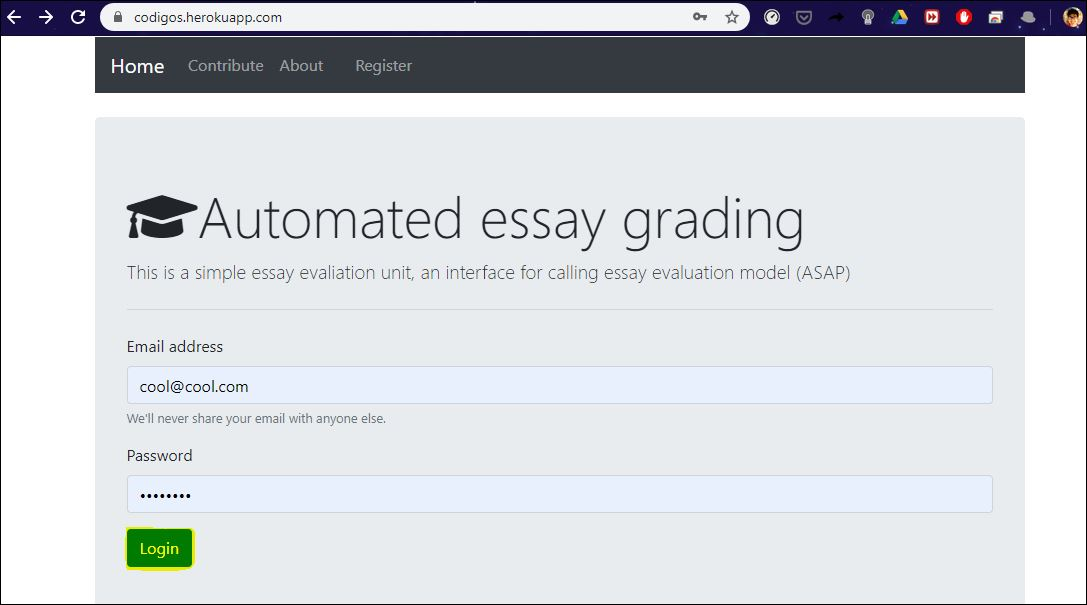
\includegraphics[width=11cm]{5}
    \caption{\label{fig:your-figure2}Login}
    \end{figure}
    \item If you have an account already, just log in and move forward to next sub section, else read on
    \item Click on register link on the navbar (in web portal) or on title bar (In android app)
    \begin{figure}
    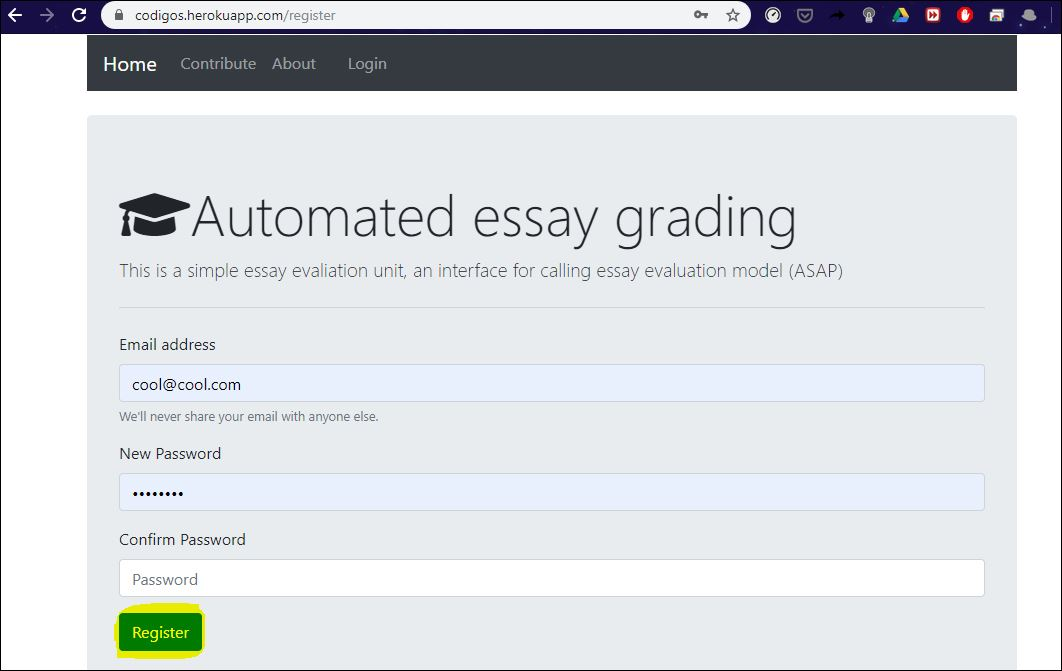
\includegraphics[width=11cm]{6}
    \caption{\label{fig:your-figure2}Register}
    \end{figure}
    \item Register by giving your details
    \item If successful, you should be re directed to the login screen
    \item Log in and move on to the next sub section
\end{itemize}
\subsection{Grade your essay}
\begin{itemize}
    \item Once logged in, you should see the main evaluation page
    \item Now, there are two options for you to get your essay validated and get it’s corresponding score
    \begin{figure}
    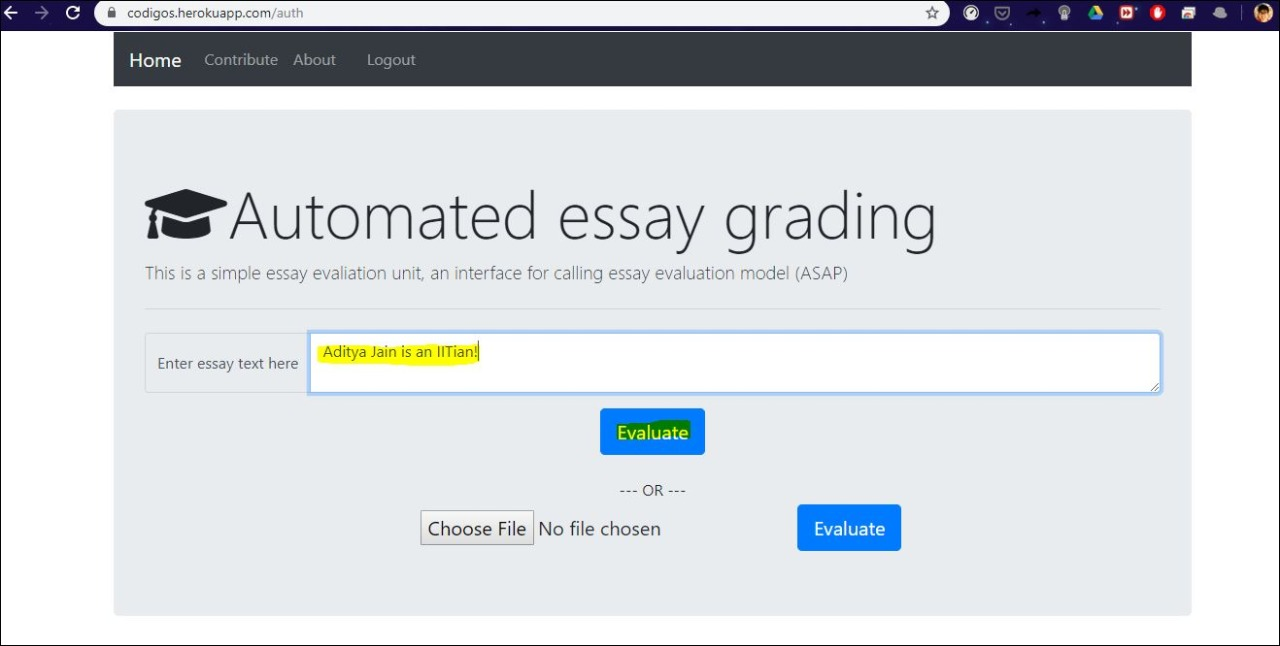
\includegraphics[width=11cm]{2}
    \caption{\label{fig:your-figure2}Evaluation}
    \end{figure}
    \begin{itemize}
        \item Typing text
            Beside "Enter essay text here”, you can directly start entering your text here or can paste it from any other source (txt, pdf, etc.)
        \item Upload file (only text)
            You can directly upload an already written essay file, by clicking on the “Upload essay” button and hence, no need to copy and paste the text onto the website.
    \end{itemize}
    \item Once done with any of the steps, just click on the “Evaluate” button and Voila!! Your Essay score is in front of you. (Evaluated on a scale of 0-100)
    \begin{figure}
    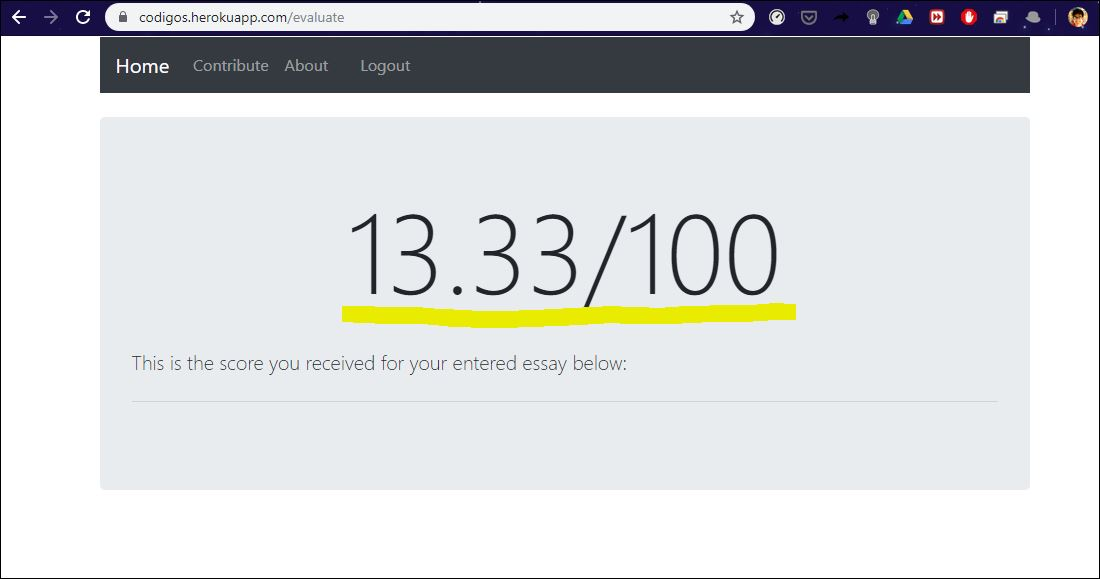
\includegraphics[width=11cm]{1}
    \caption{\label{fig:your-figure2}Score}
    \end{figure}
\end{itemize}

Note:
\begin{itemize}
    \item For getting accurate results, the input text (your essay) shall only consist of any combination of English alphabet, special characters and mathematical digits.
    \item The input text (your essay) shall consist of at least 7 words.
        Entering the text: “Aditya Jain is an IITian!”
        The text only consists of 5 words which doesn’t meet the requirement as mentioned above.
\end{itemize}
\subsection{Contribute}
Using this feature, you can contribute to our website, just to increase its accuracy and hence can avail the benefits of its accuracy later on.\\
All you need to do is:
\begin{itemize}
    \item Text of your Essay
    \item The topic of your Essay
    \item The score of the Essay evaluated by you (manual checking)
    \item Click on the Contribute! button.
\end{itemize}
\begin{figure}
    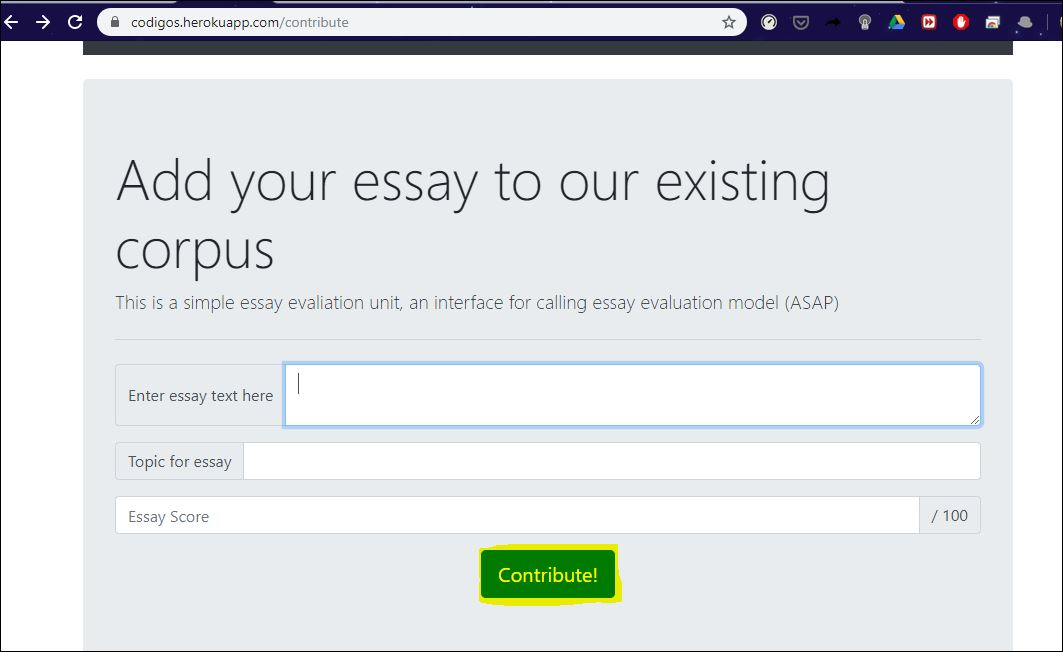
\includegraphics[width=11cm]{3}
    \caption{\label{fig:your-figure2}Contribute}
    \end{figure}
    \begin{figure}
    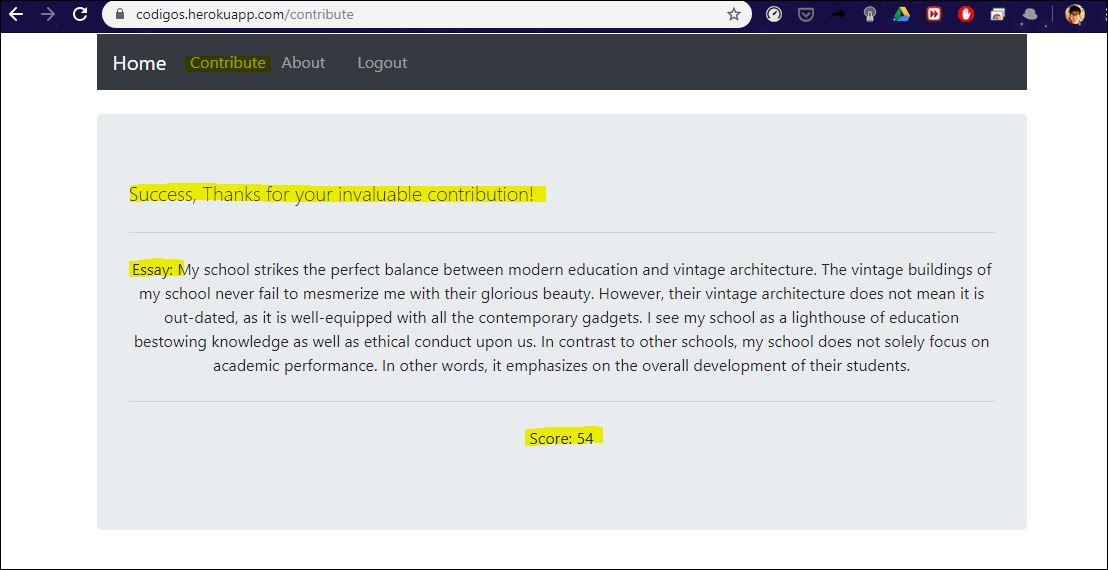
\includegraphics[width=11cm]{4}
    \caption{\label{fig:your-figure2}Thanks}
    \end{figure}
Just by completing these 3 steps, you have successfully contributed for a great cause! You are now a Codigo!

\end{document}
